%!TEX root = cscw2018-comic.tex
In this study, we investigated persuadee's preferential choice between the plain-text representation and the comic representation of persuasive messages and understood how different comic elements affect persuadee's preference. We first composed five persuasive messages in plain text form and then created their corresponding comic representation. To answer our research question, we conducted a field study on Amazon Mechanical Turk. \par
\subsection{Composing Persuasive Messages in Plain Text}
Borrowing the idea from Psychology and Behavioral Economics, the key persuasive technique we adopted here is implying social norm through the messages (e.g. how participant's friends are doing). Also, we incorporate the idea from Tversky and Kahneman that people will be influenced differently if the same message is framed as risk averse or risk taking \cite{tversky1981framing}. The main goal of all messages is the same, persuading the target persuadee to engage more exercise. The main reasons to choose this topics are 1) As a basic daily activity everyone has the need to exercise. 2) People can easily understand the message and relate to themselves. 3) Engaging more exercise is mostly based on audience own willingness instead of any other subjective resources.\par
Therefore, we created two sets of messages that either framed from a positive standpoint or a negative standpoint. The followings messages were presented in our study.\par
\textit{Positive framed persuasive messages:}
\begin{enumerate}
 \item In the past week, you spent more time at the gym than did 65\% of your friends
 \item Congrats! You have reached your goal of exercising three times a week.
 \item Over the past month, you exercised more than did 90\% of your friends.
 \item Your exercise activity is in the top 20\% of all your friends.
 \item Over the past three weeks, you went to the gym more often than 60\% of your friends did.
\end{enumerate}\par
\textit{Negative framed persuasive messages:}
\begin{enumerate}
 \item	In the past week, you spent less time at the gym than did 65\% of your friends
 \item Congrats! You did not reach your goal of exercising three times a week.
 \item	Over the past month, you exercised less than did 90\% of your friends.
 \item	Your exercise activity is in the bottom 20\% of all your friends.
 \item	Over the past three weeks, you went to the gym less often than 60\% of your friends did.
\end{enumerate}

\subsection{Generating Comics}
In this study, we create a based template for all comic messages that includes two characters in a conversation and the scenario is 'One day, your friend has something to tell you.'\par

We developed an algorithmic comic generator that based on Comix I/O, an open source project that creates comics with stick figures using HTML markup \cite{cmx.io}. To maximizing the flexibility, we further developed the existing build with Canvas and rough.js \cite{canvasjs,rough.js}. The generator allows us to create the comic representation of a persuasive message in XKCD style \cite{munroe2009xkcd} and with variations in character's gesture, inter-character distance and background shading.\par

\begin{figure}[b]
    \centering
    \begin{tabular}{cc}
    \subfloat[Three levels of gesture intensity for positive framed messages from neutral to the happiest]{\label{figur:1a}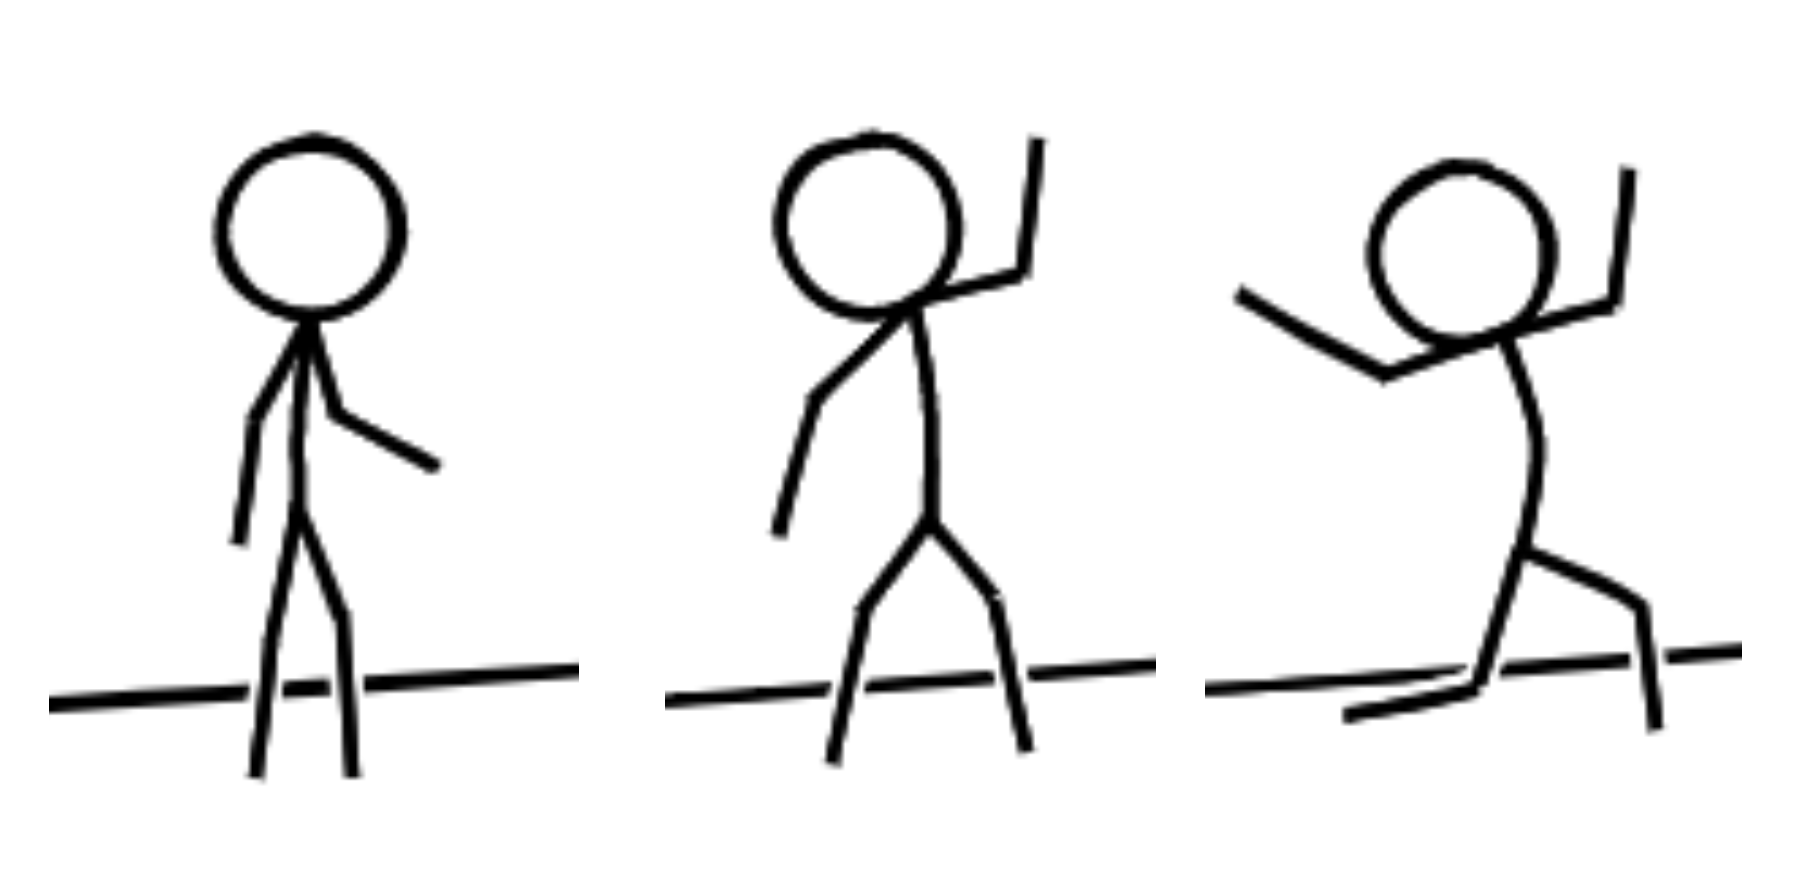
\includegraphics[width = 0.4\columnwidth]{figures/pos_figures}} &
    \subfloat[Three levels of gesture intensity for negative framed messages from neutral to the most frustrated ]{\label{figur:1b}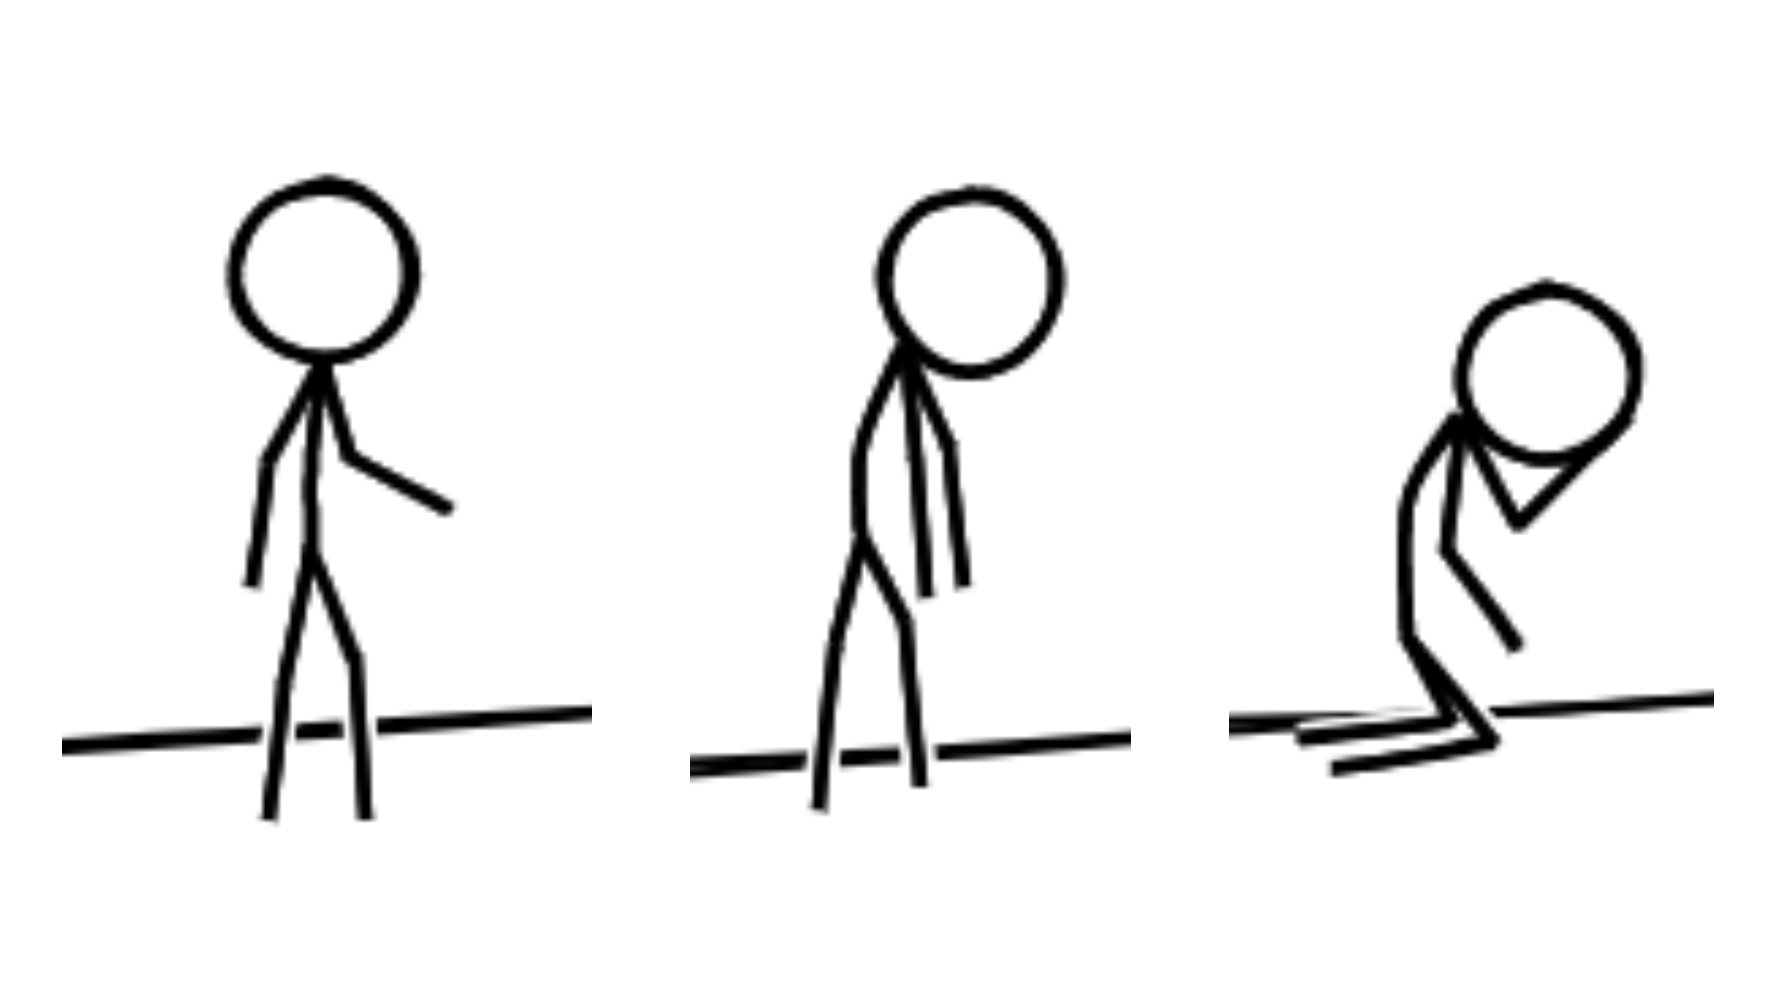
\includegraphics[width = 0.4 \columnwidth]{figures/neg_figures}}\\
    \end{tabular}
    \caption{Different character gestures to communicate various levels of emotional intensity}
    \label{figur:figures}
\end{figure}

\begin{figure}[t]
    \centering
    \begin{tabular}{ccc}
    \subfloat[Close Friends]{\label{figur:3a}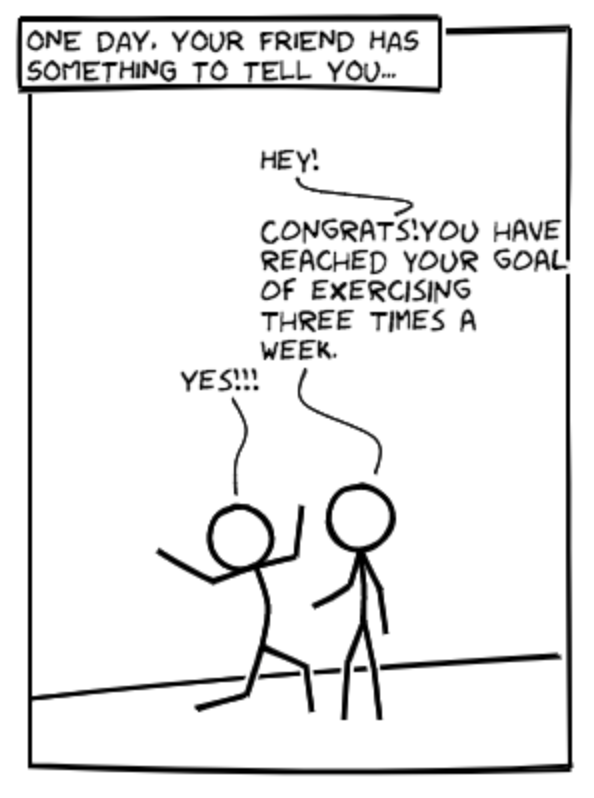
\includegraphics[width = 0.27\columnwidth]{figures/d0}} &
    \subfloat[Friends]{\label{figur:3b}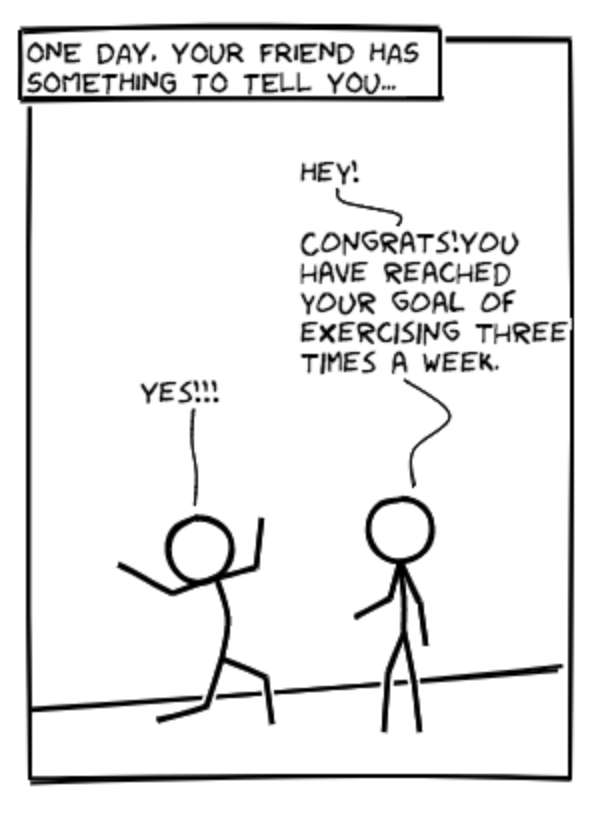
\includegraphics[width = 0.27 \columnwidth]{figures/d1}} &
    \subfloat[Acquaintance]{\label{figur:3c}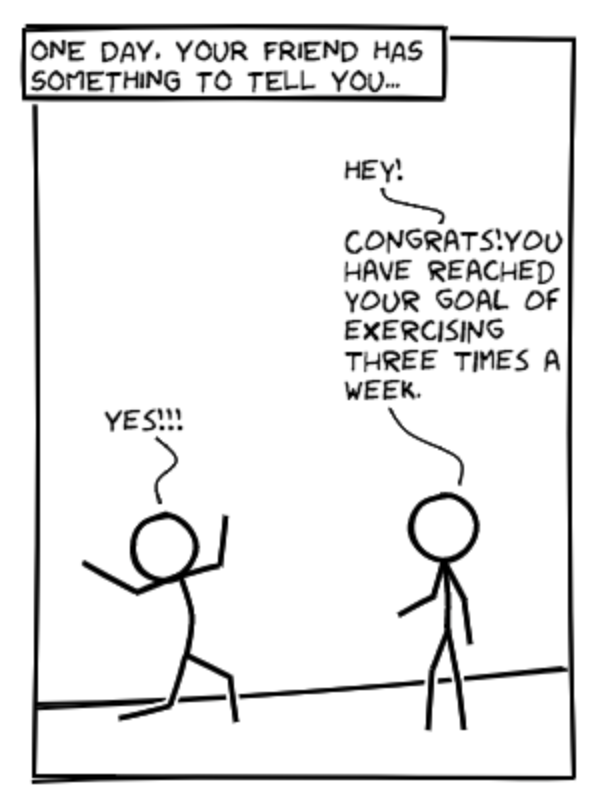
\includegraphics[width = 0.27 \columnwidth]{figures/d2}}\\
    \end{tabular}
    \caption{Different distance to communicate various levels of relationship closeness}
    \label{figur:distance}
\end{figure}

For gesture, we created the gesture library in a JSON format with two main categories: positive and negative corresponding to how the original message is framed, each with three levels of emotional intensity see Figure~\ref{figur:figures}. \par
For the distance between two character, we have three levels of variance from close to far as well. The three levels of distance represents the relationship between to characters as close friends, friends, acquaintance, from close to far, see Figure~\ref{figur:distance}. \par
For the background shading, we have a total of three levels from white to dark grey. Each level represents a level of emotional intensity, white as lowest,see Figure~\ref{figur:shading}. \par

\begin{figure}[b]
    \centering
    \begin{tabular}{ccc}
    \subfloat[Lowest]{\label{figur:4a}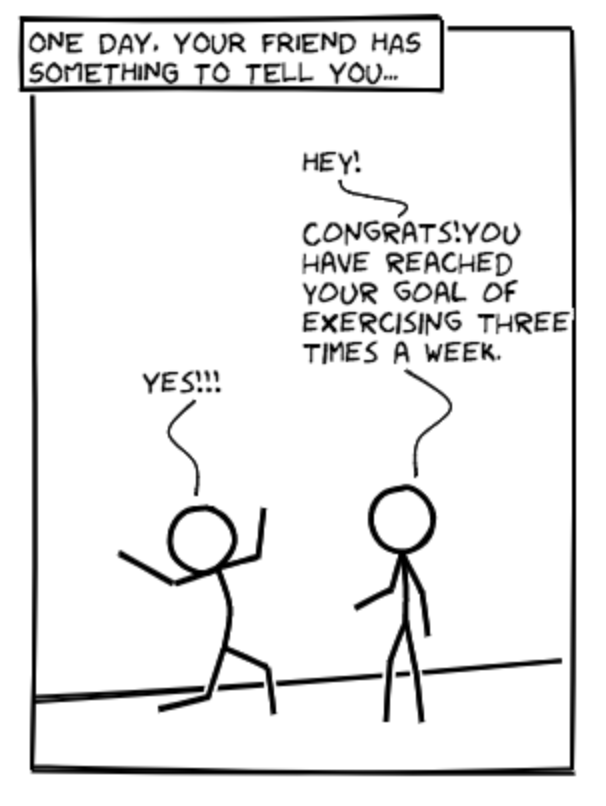
\includegraphics[width = 0.27\columnwidth]{figures/s0}} &
    \subfloat[Moderate]{\label{figur:4b}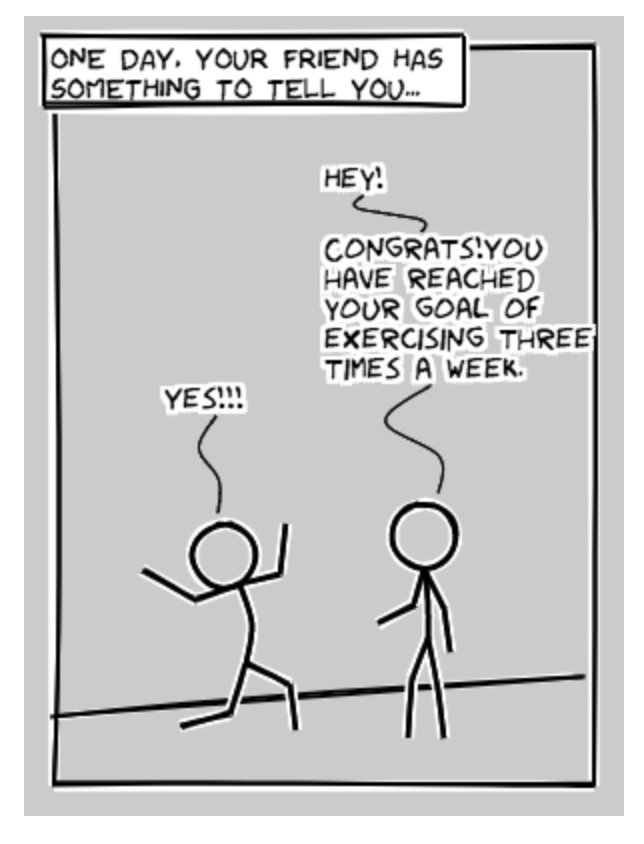
\includegraphics[width = 0.27 \columnwidth]{figures/s1}} &
    \subfloat[Intense]{\label{figur:4c}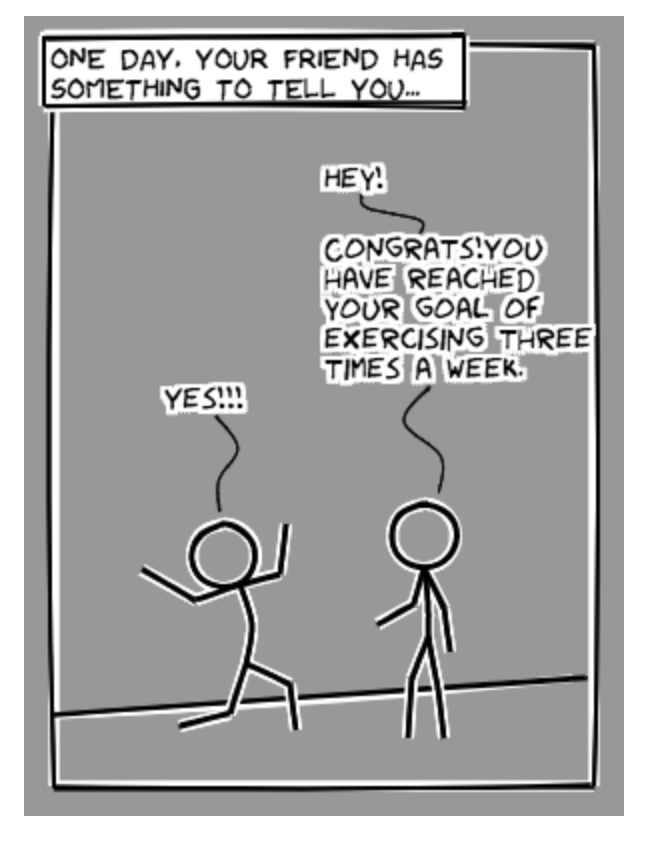
\includegraphics[width = 0.27 \columnwidth]{figures/s2}}\\
    \end{tabular}
    \caption{Different background to communicate various levels of emotional intensity}
    \label{figur:shading}
\end{figure}

To make a fair comparison between plain text representation and the comic form, the content of text information is the same in both conditions.  \par
In total, for each message we have a total of 27 variations in terms of character gesture, inter-character, and background shading. In this study, 270 comics was created corresponding to 10 plain text messages, e.g. Figure ~\ref{figur:distance},Figure~\ref{figur:shading}. \par

\subsection{Study Design}
To test our hypotheses, we designed and conducted a between-subject field study through Amazon Mechanical Turk. In the experiment, participants will see a total of five persuasive messages in both plain-text form and comic form side by side. Then, the participant will be asked which form of the message is perceived as more persuasive and how persuasive is it.\par
\textit{Experiment Procedure.} Once participants agreed to join our study, they will be randomly assigned to two conditions 1) Positive message condition where all persuasive messages are framed in a positive way and 2) Negative condition where all persuasive messages are framed in a negative way. In both conditions, participants will compare five persuasive messages.\par
For each persuasive message, the participant will compare the same message in plain text and in a comic form on a 7-item Likert scale. \par
\textit{Display Order.} To mitigate any potential bias toward the display order of the plain-text representation and comic-style representation. The display order is randomly assigned. Both plain-text representation and comic-style representation have equal chance to show on the left side.\par
\textit{Attention Checker.} To control the data quality, we embedded two attention checkers in the study. The first one appears after the third comparison and the second one shows up after the last comparison. Both attention checkers asked subjects to choose a comic that matches a simple description, e.g. "Which of the following comics has two characters?"\par
\textit{Rating Scale Design.} The 7-item Likert scale is ranging from -3 (left) to 3 (right) where 0 means neutral. The direction of the scale flips corresponding to the position of the comic and plain text, see the right part of Figure~\ref{fig:change}. \par

\subsection{Pilot Tests on the Study Design}
Before the actual experiment, we first tested our design in a small scale. We deployed our study on Amazon Mechanical Turk and received total of 10 feedbacks in 5 hours. Surprisingly, 5 of 10 participants reports the scale is confusing. 3 of them reports the flipping scale makes they spend more time on figuring out which side is which. One participants said "When I am answering my last question, I suddenly noticed the scale is different. I noticed the order of text and graph is changing but never notice the scale is changing as well. ``That's really confusing!!''\par

Based on the valuable feedback from our pilot test, we reiterated our study design. In the final design, we fixed the order of the rating scale. However, since the order is fixed, potential demand characteristics may be introduced by the scale, e.g. the researcher may want me to choose the larger number or items on the right/left side is expected. To minimize potential biases, in our final design, another layer of randomness was added. The direction of the scale no longer changes respect to the position of the messages, but the direction of the scale is randomly assigned for each participant. Also, the number on the scale is replaced by text as neutral, slightly persuasive, text/comics is more persuasive and strongly persuasive.\par

Another problem we noticed is that 3 out of 10 participants told us the text representation of the message hard to read. Therefore, we adjusted the size of the comic and text to make sure both of them have similar readability.\par

The final design is shown in left of Figure~\ref{fig:change}.Another round of pilot study with another 10 participants shows the newer design has successfully addressed the problems in the old design.\par

\begin{figure}
  \centering
  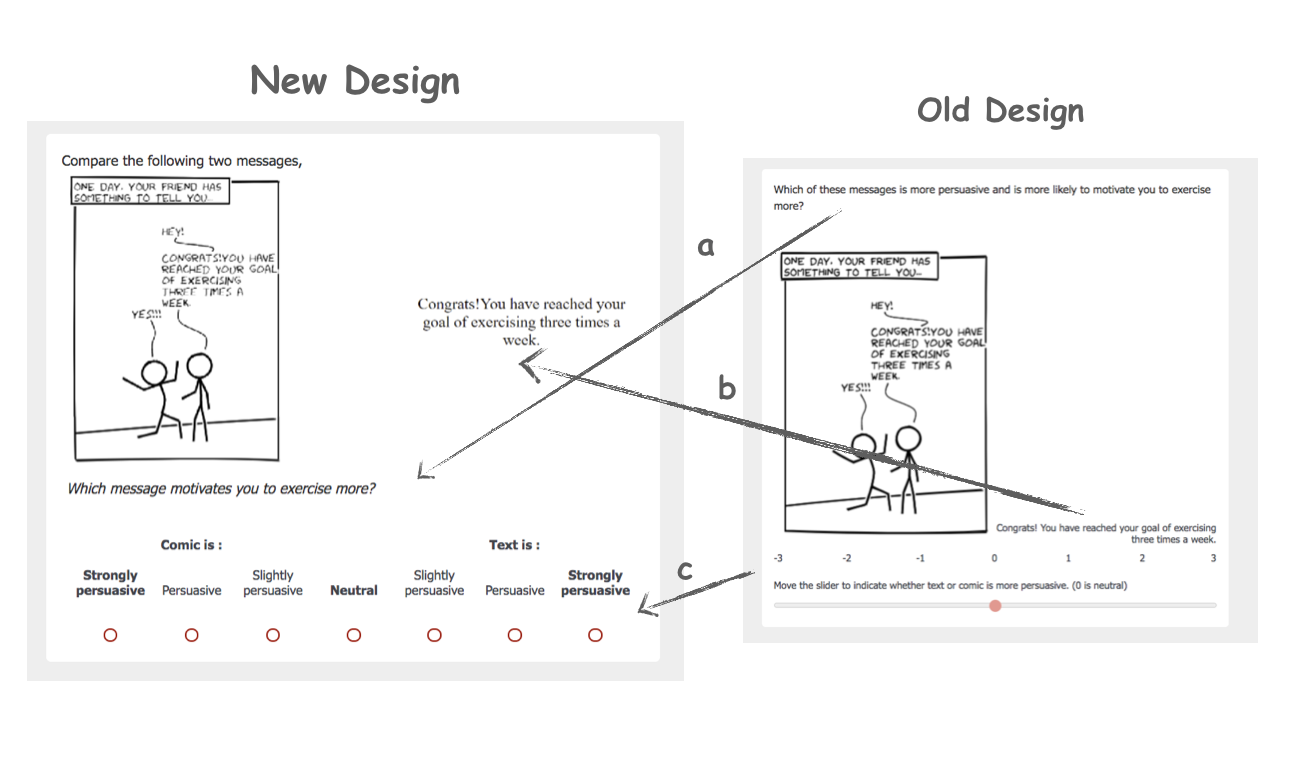
\includegraphics[width=0.95\columnwidth]{figures/change}
  \caption{Design of the task before and after the pilot study. A. Change the position of the question to make the question more clear. B. Adjust the position and the size of the text message to improve readability. C. Improve the rating scale to make it easy to interpreted.}
  \label{fig:change}
\end{figure}


\subsection{Participants}
We published our HITs on Amazon Mechanical Turk titled with "A short survey about your exercise motivation". The price tag for each HIT was \$8/hr, which were the rewards the workers would get regardless of their performance. The threshold for participant to join our study is a 95\% Approval Rate. On the HIT page, participants would see a link to our experiment site and a text input box for them to enter a six-digit completion code. Repeated worker will be rejected as we instructed in the task description.\par
